%\documentclass[review]{elsarticle}
\documentclass[5p]{elsarticle}


\usepackage{lineno,hyperref}
\usepackage[separate-uncertainty=true,multi-part-units=single,range-phrase=--]{siunitx}
\usepackage{color}
\modulolinenumbers[5]
\usepackage{mhchem}
\usepackage{enumitem}
\usepackage{trackchanges}
\usepackage{ulem}
\graphicspath{{Figures/}}

\journal{Geomorphology}



\newcommand{\COMON}{\begin{color}{blue}}
\newcommand{\COMOFF}{\end{color}}

\newcommand{\alon}{\begin{color}{red}}
\newcommand{\aloff}{\end{color}}

\newcommand{\GSon}{\begin{color}{orange}}
\newcommand{\GSoff}{\end{color}}

\newcommand{\CPon}{\begin{color}{green}}
\newcommand{\CPoff}{\end{color}}



%% APA style
\bibliographystyle{model5-names}\biboptions{authoryear}

%\addeditor{Alain}

%%%%%%%
% The trackchanges package adds five new LaTeX commands:
%
%  \note[editor]{The note}
%  \annote[editor]{Text to annotate}{The note}
%  \add[editor]{Text to add}
%  \remove[editor]{Text to remove}
%  \change[editor]{Text to remove}{Text to add}
%
% complete documentation is here: http://trackchanges.sourceforge.net/
%%%%%%%



\begin{document}


	\begin{frontmatter}

\title{Three-dimensional geophysical imaging of the Royal Arches Meadow Rock avalanche in Yosemite Valley, California}

%% Group authors per affiliation:
\author[Marcus]{Marcus Pacheco\corref{cor1}}
\address[Marcus]{Earth & Environmental Sciences, California State University, Fresno}
\cortext[cor1]{Corresponding author.}
\ead{mvpacheco90@mail.fresnostate.edu}

\author[Alain]{Alain Plattner}
\address[Alain]{2Geological Sciences, University of Alabama}

\author[Greg]{Greg Stock}
\address[Greg]{National Park Service, Yosemite National Park}

\author[Chris]{[Christopher Pluhar}
\address[Chris]{Earth & Environmental Sciences, California State University, Fresno}



										\begin{abstract}
										

Rock avalanches have occurred intermittently in Yosemite Valley, California, since the retreat of glaciers at the end of the last ice age \SI{\approx15}{\kilo a}. The Royal Arches Meadow rock avalanche is an approximately \SI{0.5e6}{m^3} deposit of rock debris located in eastern Yosemite Valley. Cosmogenic beryllium-10 exposure ages of boulders on the deposit indicated that the rock avalanche occurred at \SI{14+-0.3}{\kilo a}, shortly after deglaciation. The interface between the rock avalanche deposit and the underlying fluvial, deltaic, and lacustrine sediments therefore provides a reference for the valley surface at that time. To investigate amd locate this interface, we collected eight Ground Penetrating Radar (GPR) and five Electrical Resistivity Tomography (ERT) profiles longitudinally and transversely crossing the rock avalanche. Both methods are sensitive to the contrast between the granitic avalanche deposit and the underlying sediments. We identified multiple reflectors in the GPR data that are continuous across the profiles, while ERT inversion results along the same profiles showed resistive material (\SIrange{1000}{8000}{\ohm.m}) overlying relatively conductive material (\SI{<1000}{\ohm.m}). By constraining ERT inversions with picked GPR reflectors, we identified a single GPR reflector that separates resistive material on top from relatively conductive material underneath. This reflector is approximately horizontal at an average elevation of ~1207 m. We interpret this interface as the bottom of the rock avalanche and hence as the surface of Yosemite Valley at the end of the last glaciation. Thus, we estimate that \SI{10}{m} of total aggradation have occurred on the terrace adjacent to the rock avalanche since emplacement. Our findings collaborate with the reconstruction of the sedimentation history and landscape evolution of Yosemite Valley. Moreover, the identification of bottom of the RAMRA using geophysical methods, provided us insights into how to imrpove volume estimation for similar deposits.     
y.

									\end{abstract}

					\begin{keyword}
GPR \sep ERT \sep Yosemite
%\texttt{elsarticle.cls}\sep \LaTeX\sep Elsevier \sep template
%\MSC[2010] 00-01\sep  99-00
					\end{keyword}

	\end{frontmatter}

%\linenumbers






\section{Introduction}

Large rock slope failures such as rock avalanches are among the most efficient processes changing mountainous landscapes \COMON (REFERENCES HERE) \COMOFF. In Yosemite Valley, California, rock slope failures not only poses a serious hazard to the nearly four million yearly visitors, but also to the park infrastructure. In this project, we explore (describe?) how we used one of those large rock slope failure deposit in the valley, to gain insights into the local sedimentation history and landscape evolution. 

In Yosemite Valley, postglacial massive rock debris deposits  are well preserved \COMON (REFERENCE HERE) \COMOFF, and can provide us with a position marker of the valley floor during the time that they occurred. 

Unlike Rockfall, which happen very frequently in the park and produce small volume of debris, rock avalanches are rare, and typically move large masses of material over long distances in a matter of seconds (Stock and Uhrhammer, 2010). Consequently, these events are an important geomorphic process reshaping the landscape of Yosemite Valley. Postglacial massive rock debris deposits, such as rock avalanches,  are well preserved in Yosemite Valley \COMON (REFERENCE HERE) \COMOFF, and can provide us with a position marker of the valley floor during the time that they occurred


\subsection{Physical Setting}

Yosemite Valley was initially carved by fluvial incision, and latter deepened by several glaciation cycles over the past few millions of years. The most recent glaciation, locally known as Tioga glaciation, peaked between \num{28000} and \num{17000} years BP and only partially filled  Yosemite Valley (\cite{huber1987geologic}). Subsequently, Yosemite Valley is thought to have been deglaciated somewhen between \num{15000} and \num{17000} years ago (\cite{huber1987geologic};  \cite{Wieczorek+1996}.

The valley fill is mainly composed of lacustrine, deltaic, and fluvial sediments \COMON Reference here\COMOFF, has a depth of up to \SI{600}{m} \cite{gutenberg1956seismic}, and the current valley surface is a broad and flat flood plain meandered by the Merced River \cite{Wieczorek+1996}. Flanked by up to \SI{1000}{m} tall and steep granitic rock faces (\COMON Stock and Uhrhammer, 2010 \COMOFF).
    
    
    
\subsection{Slope Failures In Yosemite Valley}

Because of  the nearly vertical and sometimes overhanging walls, slope failures events such as rock falls, rock slides, and debris flows are common in Yosemite Valley. Most of those deposits are concentrated relatively close to the cliffs where they originated. However, at ten locations in Yosemite Valley , rock debris have traveled hundreds of meters onto the valley \COMON(REFERENCE HERE)\COMOFF. Those deposits were termed Rock Avalanches, because of their distinct hummocky morphology, run out of hundreds of meters, and volumes in the hundreds of thousands of m3 \COMON(Stock 2014, Evans 2006,  Hungr 2014, Wieczorek 1998, Stock 2010, Stock 2011)\COMOFF. 


\subsection{Royal Arches Meadow Rock Avalanche}\label{sec:introRAMRA}

The Royal Arches Meadow Rock Avalanche (RAMRA) lies in the eastern Yosemite Valley, inside Yosemite National Park in California, USA.


								   \begin{figure*}[h]

	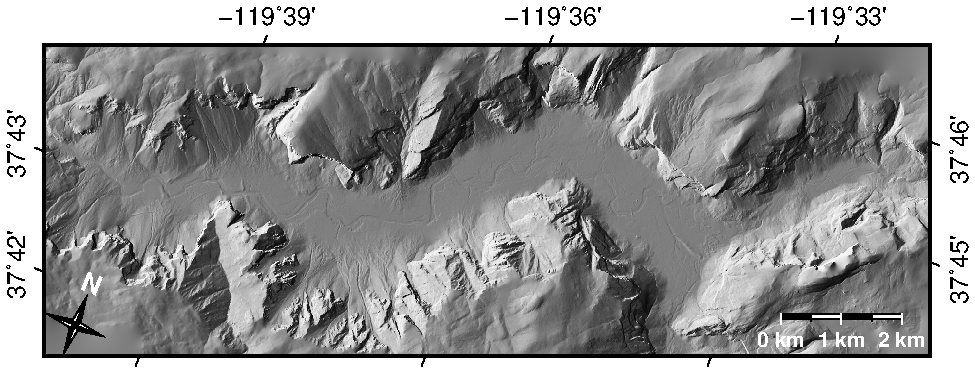
\includegraphics[width=\textwidth]{Yosemite.pdf}
		\caption{: Yosemite Valley Map View, white star highlight the study area.  \label{Study_Area}}

								   \end{figure*}



The RAMRA has a exposed runnout of approximately 180 m onto the valley, and boulders ranging from tens of centimeters to several meters tall (Fig.~\ref{Study_Area2} A and B). Generally, the size of the boulders decrease away from the cliff face toward Tenaya Creek in southwestern direction (Fig.~\ref{Study_Area} C and D).



                             \begin{figure*}[h]

  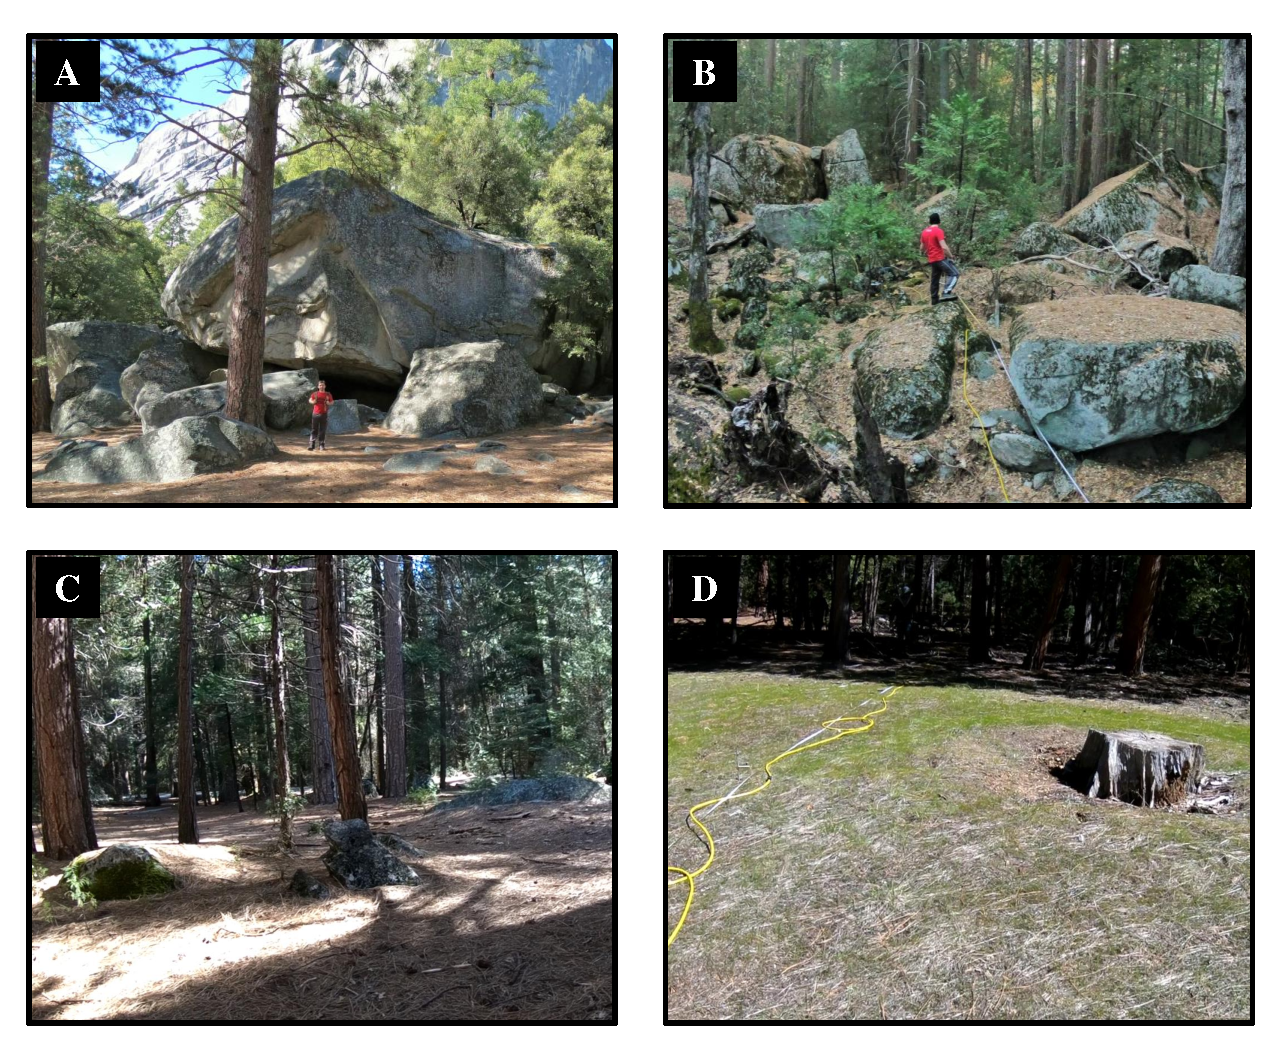
\includegraphics[width=\textwidth]{Study_Area2.pdf}
  \caption{ Pictures of the study area from proximal do distal - (A) and (B): Large boulders in the proximal part of the avalanche, (C) distal portion of the rock avalanche, (D) absence boulders on the surface closer to the Tenaya creek cutbank. 
  \label{Study_Area2}}
  
                            \end{figure*}



Cosmogenic \ce{^{10}Be} exposure ages demonstrate that the Royal Arches Meadow Rock Avalanche happened 14,030 ± 340 BP \COMON[XXX citation XXX]\COMOFF. This makes the RAMRA the oldest avalanche in the park. More importantly, because this event happened shortly after the LGM in the valley, the interface between the bottom of the RAMRA and the underlying paleo-valley marks the elevation state of the valley shortly after the LGM (15000 year B.P.). This boundary represent an important marker to understand the sedimentological and landscape evolution of the valley, and therefore it is tour target of study. Because this interface is not exposed in the surface, we combined geophysical methods to locate the position of the bottom of the RAMRA in subsurface, and used Cosmogenic beryllium-10 ages to estimate the age of the avalanche, and therefore  gain insights into the rates of local deposition.

% * <marcus vinicius Pacheco> 21:07:12 18 Jan 2020 UTC-0800:
% Hi Greg, I was previously using the age of the RAMRA to link it with the LGM, and to provide some closure to the intro by stating our goals. However, now that we are including the ages in the paper, I wonder if there is a better way to phrase it here without being repetitive, but at the same time keeping the essential idea.


\bigskip

                 
                 
\subsection{Geophysics and Slope Failures Deposits}

To obtain spatially continuous information of the bottom of the RAMRA, we used a combination of two non-intrusive geophysical methods. Electrical Resistivity Tomography (ERT) and Ground Penetrating Radar (GPR). Geophysical methods have been successfully applied to image slope failures deposits (e.g., \cite{sass2006determination}; \cite{otto2006comparing}; \cite{socco2010geophysical}; \cite{brody2015near},\cite{liu2018near}), highlighting the efficiency of combining GPR and ERT.
                 
Ground Penetrating Radar is a geophysical technique that detects electrical discontinuities in the shallow subsurface (typically < 50 m) \citep{neal2004ground}. The most common form of GPR measurements, called common offset profiling, involves keeping a transmitter antenna and a receiver antenna at a fixed distance and moving them along a profile line on the surface to detect reflections from subsurface features \citep{jol2008ground}. Abrupt changes in dielectric permittivity caused by different lithologies, but also variations in grain size, and even grain orientation can reflect GPR waves (Olhoeft, G. R., 1998 and \citep{neal2004ground}. Therefore, we expect the contact between the bottom of the RAMRA with the underlying sediments to create strong reflections which can be detected by the GPR.          

Electrical Resistivity Tomography operates by measuring voltage differences caused by electric currents that are injected into the ground. Overlapping measurements can then, with the help of computational inversions, be turned into images of the electrical resistivity variation within the subsurface. These procedures are typically underdetermined. We hence can greatly improve the reliability of our solutions by providing additional constraints in the form for example of known interfaces (Oldenburg 1999; Loke 2013). We expect that this interface to be marked by a strong contrast in electrical resistivity, because the rock avalanche is composed of mostly granitic debris (clast supported matrix), while the palleo-valley surface sediemnts are mostly composed of silt, clay, fine sands and palleo-soil. 

\COMON Doetsch, Linde, Pessognelli, Green, \& Günther, (2012)\COMOFF, have demonstrated the effectiveness of using Ground Penetrating Radar reflectors to constrain electrical resistivity tomography (ERT). This technique operates by offering the option of removing smoothness across the interfaces identified in the GPR data in the ERT inversion \COMON + add more references here! \COMOFF.  



\bigskip   



\section{Methods}

\subsection{Geophysics}

\alon The large area of the rock avalanche and limited accessibility
due to large boulders and vegetation (Fig.~\ref{Study_Area2}B) made a
full three-dimensional investigation impossible. Initial investigation
of the rock avalanche led to an outline that follows the topographical
expression of the rock avalanche. Due to the age of the rock
avalanche, and its location close to a sediment-rich stream, we can
not exclude the possibillity that the rock avalanche has been partially covered by post glacial aggradation. 
sediments. \aloff We therefore collected eight Ground Penetrating Radar
(GPR) and five Electrical Resistivity Tomography (ERT) profiles
longitudinally and transversely crossing the rock avalanche
\COMON(Figure - Map)\COMOFF, covering both exposed parts of the rock
avalanche, and the adjacent area.

%% I THINK THE FOLLOWING COULD BE EXPLAINED IN THE RESULTS OR
%% INTERPRETATION PART OF THE PAPER:  Because the extent of the rock
%% avalanche is unknown, we positioned several profiles inside the
%% exposed portion of the rock avalanche. This way, we insured that we
%% would be undoubtedly imaging the rock avalanche deposit just
%% beneath the surface, and possibly its bottom. On the other hand,
%% extending the geophysical profiles beyond the exposed portion of
%% the rock avalanche, allowed us to verify the lateral continuation
%% of the bottom of the rock avalanche beyond its exposed portion.


For the GPR profiles, we used a Sensors \& Software PulseEKKO Pro (\SI{50}{\mega Hz}) system (Fig.~\ref{GPR_ERT_MapT}A) during the
months of September and October of 2018. We processed these profiles using GPRPy
\citep{plattner2019comunity,Plattner2019}, applying a time zero
correction, filter (dewow and mean trace removal), T-power gain, f-k
migration \citep{stolt1978migration} and topographic correction. We used a single velocity that we obtained from a wide angle
reflection and refraction survey on site. Raw data and GPRPy
processing scripts are included in the supplemental material of this
article. We then used the processed profiles to track the lateral continuity of specific reflectors between the profiles following the methodology proposed by
\citep{mitchum1977seismic}.



\alon passive voice... \aloff
% * <marcus vinicius Pacheco> 18:48:30 18 Jan 2020 UTC-0800:
% hi Alain, I agree with you that active voice sounds better than passive. I try to mix both to make the reading more smooth, and therefore avoid repeating "we... we... we... several times. But I can make sure that all sentences are in active, if you believe that it would sounds better.
Five ERT transects were collected at the study area (Fig.~\ref{GPR_ERT_MapT}B), using the Advanced Geosciences Inc SuperSting R1 (28 electrodes), with an electrode spacing of six meters, and a Wenner–Schlumberger and dipole-dipole acquisition scheme. Subsequently, the ERT data were filtered using DC2DInvRes \COMON (REFERENCE) \COMOFF and inverted using BERT/GIMLi (\cite{gunther2006three} and (\cite{Ruecker2017}).


								 \begin{figure*}[h]

	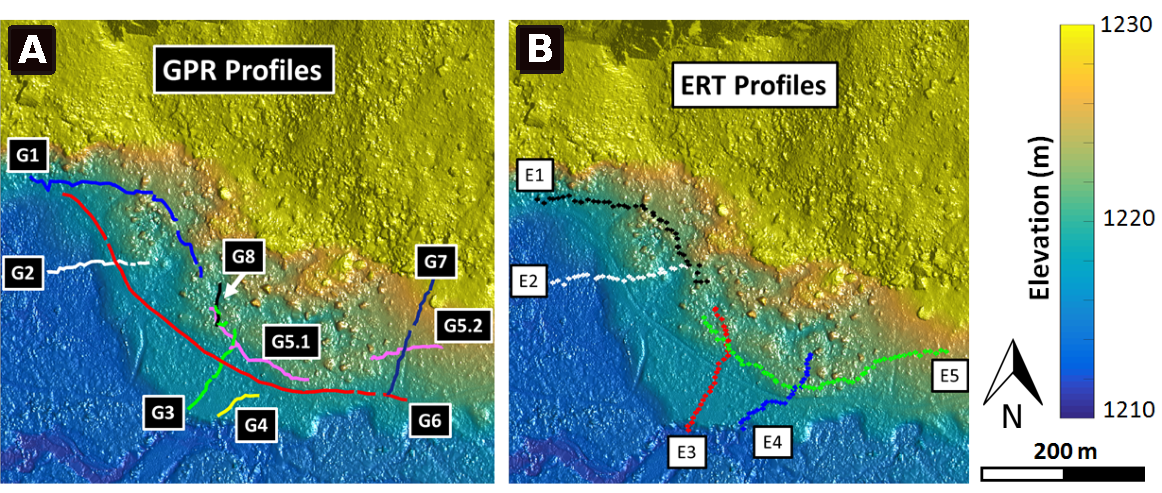
\includegraphics[width=\textwidth]{Figures/GPR_ERT_Map.pdf}
		\caption{:(A) Map view of GPR profiles, and (B) map view of ERT profiles. \label{GPR_ERT_Map}}

								   \end{figure*}



\subsection{Cosmogenic beryllium-10 exposure ages}
\alon I would use a different title for this subsection. Perhaps:
``Rock avalanche age'' or so. \aloff

-Cosmogenic be 10 in 3 locations
-Cosmogenic beryllium-10 ages yield a mean exposure age of 15.3 +- 1.4 ka


\bigskip  

 
\section{Results}


\subsection{GPR Results}

\alon Here you need to include the velocity analysis. Perhaps also put
its coordinates on the map.\aloff

% * <marcus vinicius Pacheco> 19:19:16 18 Jan 2020 UTC-0800:
% Hi Alain, I am afraid that if we include the position of the WARR on the map it is going to get even more polluted.

% * <marcus vinicius Pacheco> 19:28:57 18 Jan 2020 UTC-0800:
% -I cannot explain how we did the velocity analysis/found the velocity, on the results. Because such explanation on how to do should go on methods, as this section should be limited to what we found (results). 
% - I was also thinking that just stating: "we found 0.11 m/ns for the velocity (which I agree is a result) would not  be so relevant for the readers of this journal. 
% -So, I was wondering if it would make sense to briefly state on the methods: "we used velocity 0.11 m/ns based on the WARR data aquired...etc..." and create a section in the Discussion to talk about how finding the correct velocity inpact the data and its ncertantiesnties. (pleas advise).


We observed the following patterns of reflection in the GPR profiles: (A) from the surface until approximately 1212m of elevation, the GPR profiles are marked by a plan-parallel to sub-parallel reflectors. Varying from 12YY until 12XX m of elevation, a strong plan-parallel reflector (Alpha) is visible in all GPR profiles. (B) Bellow ~1212 m of elevation, the pattern of reflectors change to a chaotic geometry as the signal gets scattered, this pattern is limited at bottom  by a nearly horizontal reflector (Beta)  at the elevation of ~1207 m. Lastly, in profiles Gx,  Gy, Gz, another strong continuous reflector is identified at the elevation of ~1205m (Gamma) (Fig.~\ref{GPR_Oblique} A). 
The reflectors termed by us here as Alpha, Beta and Gamma appear in most of the GPR profiles and their elevation in information is described in details in Table 1. 



								 \begin{figure*}[h]

	\includegraphics[width=\textwidth]{Figures/GPR_Oblique.pdf}
		\caption{:(A) Oblique view of GPR profiles looking towards NW, (B) Tracked Reflectors Alpha, Beta, and Gamma, and (C) Interpolated surface for reflector Beta. \label{GPR_Oblique}}

								   \end{figure*}
								   
\begin{itemize}
    \item Table 1 here
\end{itemize}			   

								   
\subsection{ERT Results}

We observed  in the ERT inversion results relative resistive material (1k-8k ohm m) overlying relatively conductive material (<1k ohm m). The ERT inversions using GPR reflectors for profiles E1, E2, E3, E4 and E5 have demonstrated that Reflector Beta best constrained the inversion, by creating a sharp interface between resistive/conductive material.


\COMON Pictures? \COMOFF


\COMON Combining the Methods \COMOFF
% * <marcus vinicius Pacheco> 20:11:23 18 Jan 2020 UTC-0800:
% Hi Alain, giving the public for this journal, do you believe that worth it to still include this section exploring the reasons for the gaps in the data? I have been reading those buller points, and I think it is just going to cause a twist in the readers mind. please advise.

--Because of the difficulties imposed by the field of study (e.g. big boulders,  large fallen trunks) we were not able to collect a dense grid of geophysical data on the top of the rock avalanche. 

--We tried to collect as much geophysical data on the top of the rock avalanche as possible. However, difficulties imposed by the filed area, such as the dense presence of large boulders and/or big fallen trunks made the logistics for either GPR and/or ERT not practical. 

-To overcome the lack of one of the methods in specific locations we used the overall pattern of observation to predict how the data would look like in this area. 

- For example, we were not able to cover E5 entirely with GPR profiles, but we have a good idea where the elevation of the main reflectors would appear in this portion based on the elevation where they appear in the adjacent profiles.

-Similarly, in profile G5.1, we observed a strong signal attenuation below the elevation of 1212 m (Figure XX A). But we feel confident to picked the reflector named Beta here at the elevation of ~1207 meters based on: 
1) the weak rflction that appear among the attenuated signal at this elevation (Figure XX B).

2) the consistence in which Beta appears in the adjacent profiles at the elevation of approximately 1207m.

3) how well this picked reflector constrains the resistive/conductive transition at elevation of 1207m (Fig. XX C and D), annalagous to the other ERT constrained inverstions. 
								   
				(Fig.~\ref{Combined_ABCD})			

                                \begin{figure*}[h]

	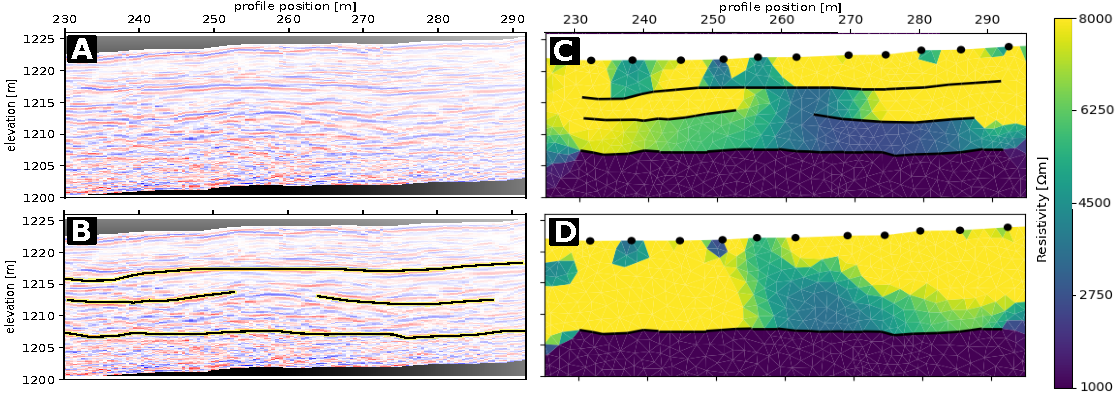
\includegraphics[width=\textwidth]{Figures/Combined_ABCD.pdf}
		\caption{:(A) Oblique view of GPR profiles looking towards NW, (B) Tracked Reflectors Alpha, Beta, and Gamma, and (C) Interpolated surface for reflector Beta. \label{Combined_ABCD}}

								   \end{figure*}


\bigskip  


\section{Discussion}

Based on the interpretation of the geophysical results, Beta interface (Fig.~\ref{GPR_Oblique} B) is the best candidate as bottom of the Royal Arches Meadow Rock Avalanche for the following reasons: 


(I) remove smoothness (ERT inversion + GPR)


(II) Reflector configuration: A) reflectors dipping, scatter of energy 

	(1) This is the Reflector that best constrain the ERT Inversion (transition between resistive / 	conductive) is the interface between the bottom of the rock avalanche


- Discuss reflector configuration (dipping, energy scatter, etc) 


- Proxy for the palleo-valley (paleoelevation)  surface of yosemite valey shortly after the last glacial maximum (LGM).



\subsection{Aggradation Rate since the LGM}

We interpret this interface as the bottom of the rock avalanche and hence as the surface of Yosemite Valley at the end of the last glaciation; thus,   10 m of fluvial sedimentation has occurred at this site over the past 14 ka


\subsection{Uncertanties}

 
%% For a subsurface velocity to distinguish individual layers) is \COMON XXX m\COMOFF. We
%% estimated it using a velocity of 0.11m/ns (extracted from WARR data),
%% a 50MHz frequency (used antenna), and the rule of thumb that vertical
%% resolution is typical equals to a quarter of the wavelength. This
%% estimation is useful to give us an idea of vertical resolution, but it
%% still an approximation, since the physical properties of the medium
%% (e.g. dielectric permitivity, electrical conductivity, and magnetic
%% permitivity) can influence the vertical resolution \COMON (Cite
%% Olhoeft, G. R., 1998, Olhoeft, G. R., 1999; \citep{neal2004ground})
%% \COMOFF.



\subsection{Volume}

-Distal volume estimation considering the bottom of the rock avalanche as the present valley floor =  378,000 m3

-Distal volume estimation considering the bottom of the rock avalanche as the interpreted bottom of the rock avalanche from the geophysical data = 955,000 m3 

-This is not the total volume of the avalanche, but it demostrate how estimations based on purely surface intereprations can be off. Mainly in environments dominated by aggradation. 


\bigskip  


\section{Conclusions}

-The combination of GPR and ERT has proven to be a powerful tool to image the interface between the RAMRA and the underneath valley sediments. 


-GPR resolution along with GPR and ERT depth sounding was satisfactory considering the goal of this project. 

-Geophysical data was consistent.
	-Different and isolated data processing show similar results when comparing different profiles and different methods. 


-rock avalanche risk assessment improvement 
	volume estimation based on purely surficial data might lead reasearchhers to underestimation


\section{acknowledgements}






\bibliography{mybibfile}

\end{document}
